%# -*- coding:utf-8 -*-
\section{研究背景}

\begin{frame}
\begin{itemize}
\item \textbf{问题背景}
\begin{itemize}
\item 设计并实现计算机辅助冠状动脉介入术仿真训练系统
\end{itemize}
\end{itemize}
\begin{itemize}
\pause \item \textbf{研究目的}
\begin{itemize}
\item 研究创建上述系统中虚拟人体解剖环境的技术方法
\end{itemize}
\end{itemize}
\begin{itemize}
\pause \item \textbf{研究内容}
\begin{itemize}
\item 基于真实病例体数据创建人体心血管系统模型的方法
\item 面向交互仿真的血管模型优化方法
\item 面向仿真训练的血管模型几何信息提取方法
\end{itemize}
\end{itemize}
\end{frame}

\begin{frame}
\begin{itemize}
\item \textbf{冠心病的严重性~[WHO(2008)]}:
\begin{itemize}
\pause \item 冠心病是全世界人口的首要死因
\item $2008$年,死于冠心病的总人数达$1,730$万
\item 超过$80 \%$的冠心病病例居住在发展中国家
\item 到$2030$年,全世界将有近$2,330$万人死于冠心病
\end{itemize}
\end{itemize}
\begin{itemize}
\pause \item \textbf{冠心病的主要成因}:
\begin{itemize}
\item 吸烟,缺乏体育运动,不健康的饮食习惯,超重和肥胖等
\end{itemize}
\end{itemize}
\end{frame}

\begin{frame}
\begin{itemize}
  \item \textbf{冠心病病理}: 
  \begin{enumerate}[A]
    \item 由于冠状动脉中血流受阻,导致自受阻位置以下的心肌长期缺氧,最终使其坏死
    \item 受阻冠状动脉的内部情况,斑块固着于血管内壁,致使血管横截面积明显缩小,血流受阻
  \end{enumerate}
\end{itemize}
\begin{figure}[t]
\centering
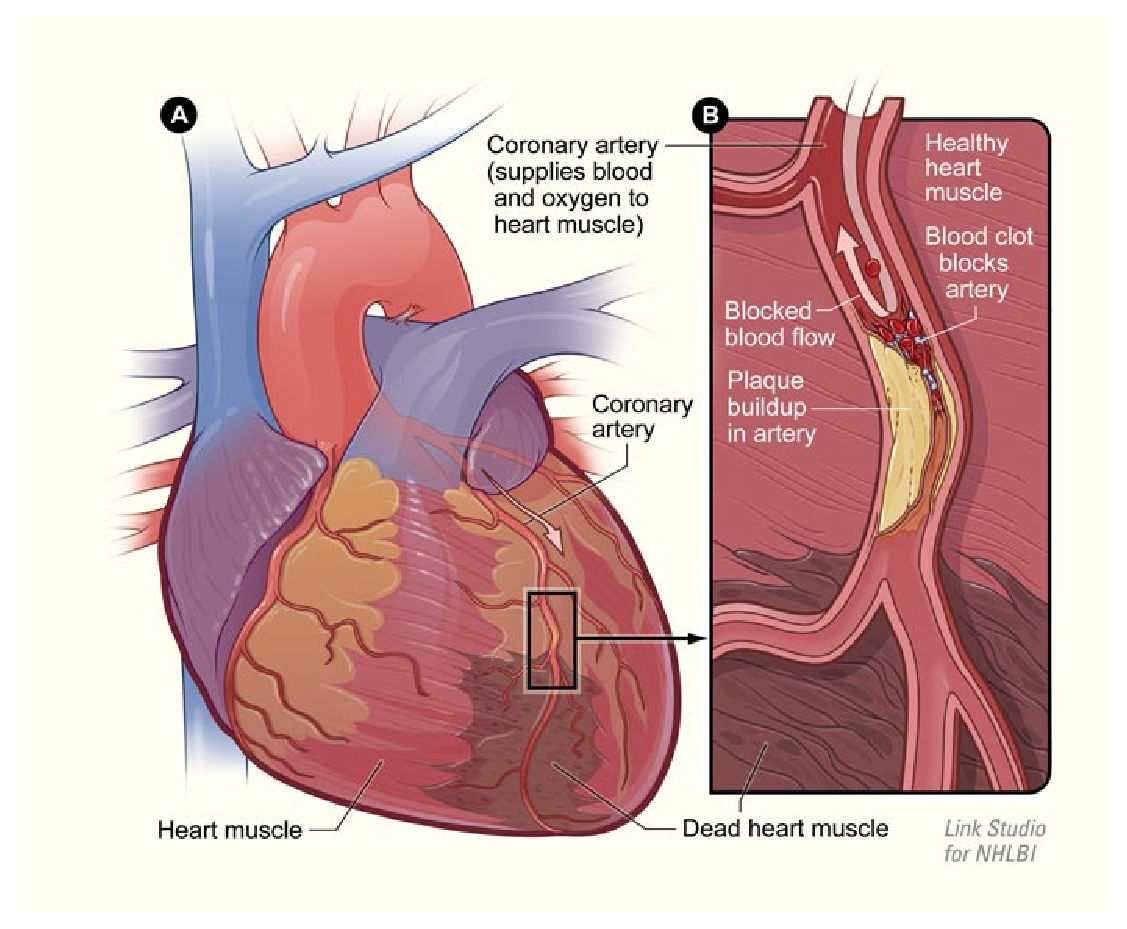
\includegraphics[height=120pt]{../../Figures/background/heart_attack_large.eps}
\caption[冠心病病理]{图片来自:\url{http://www.nhlbi.nih.gov/index.html}}
% \label{fig:heart_attack}
\end{figure}
\end{frame}

\begin{frame}
\begin{columns}[onlytextwidth]
\begin{column}{0.4\textwidth}
\begin{figure}[t]
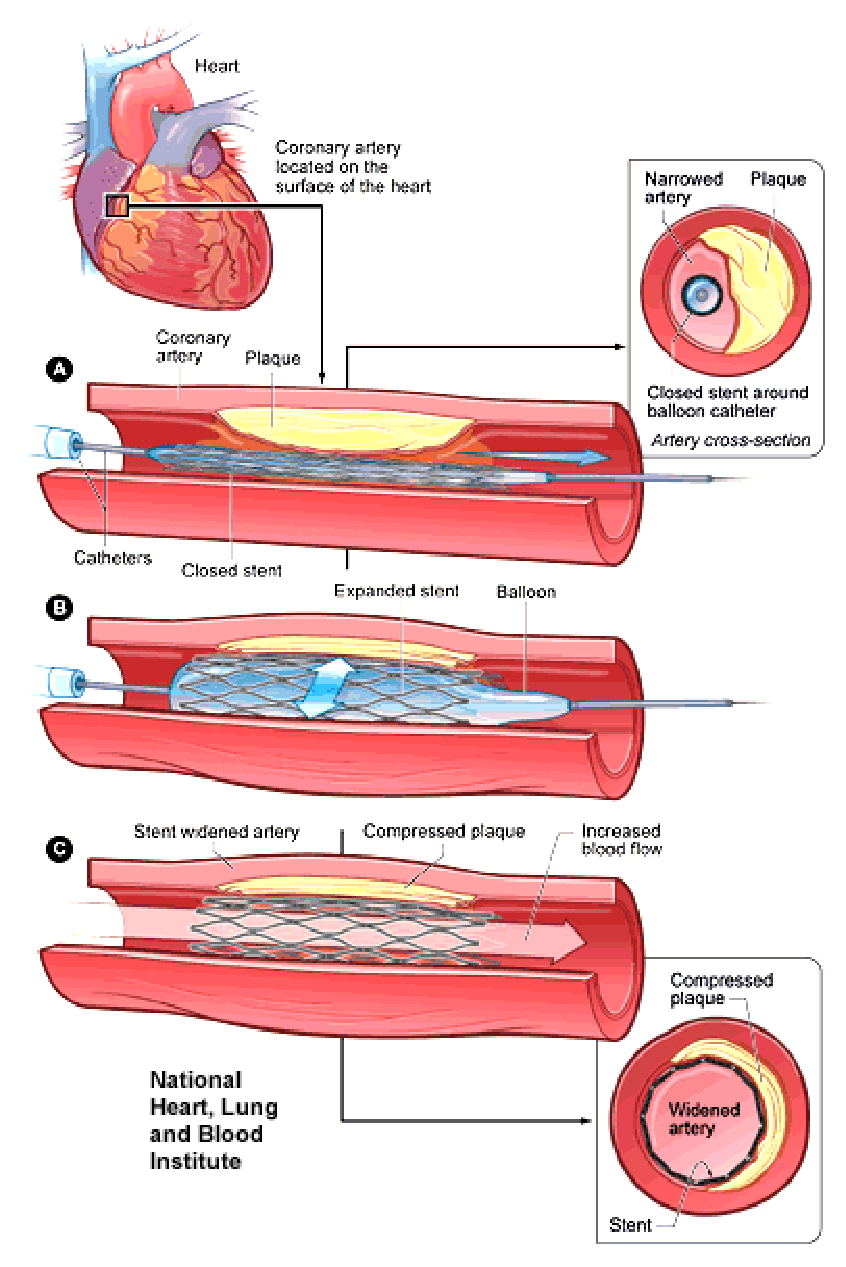
\includegraphics[height=170pt]{../../Figures/background/phauthuatmachmau_stent.eps}
\caption[冠状动脉介入术]{图片来自:\\\url{http://www.nhlbi.nih.gov/index.html}}
\end{figure}
\end{column}
\begin{column}{0.5\textwidth}
\begin{itemize}
\item \textbf{冠状动脉介入术}: 
\begin{itemize}
\item \footnotesize{重建冠脉血运的微创介入手术}
\end{itemize}
\item \textbf{主要步骤}:
\begin{enumerate}[A]
\item \footnotesize{将载有气囊的导管沿主动脉送至病灶位置}
\item \footnotesize{向气囊注入空气使其膨胀,迫使气囊外的支架扩张}
\item \footnotesize{通过导管抽出气囊内的空气使其收缩后撤出人体}
\end{enumerate}
\end{itemize}
\begin{itemize}
\pause \item \textbf{相较于传统手术的优势}
\begin{itemize}
% \setlength{\itemindent}{-.1in}
\item 创口微小
\item 痛苦减轻
\item 较短的手术时间
\item 并发症发生率降低
\item 术后恢复快
\end{itemize}
\end{itemize}
\end{column}
\end{columns}
\end{frame}

\begin{frame}
\begin{itemize}
  \item \textbf{“师傅-学徒”模式的医疗教学}: 
  % \begin{enumerate}[A]
    % \item 手工技艺的传承
    % \item 医学技术的传承
  % \end{enumerate}
\end{itemize}
\onslide<1-5>
\begin{figure}
% \begin{minipage}[t]{0.8\linewidth}
\centering
% top
% \subfigure[]{
% 
\includegraphics[height=60pt]{../../Figures/background/220px-Apprenticeship.eps}
% \quad
% 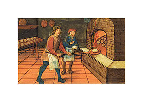
\includegraphics[height=60pt]{../../Figures/background/220px-Medieval_baker.eps}
% }
% bottom
% \subfigure[]{
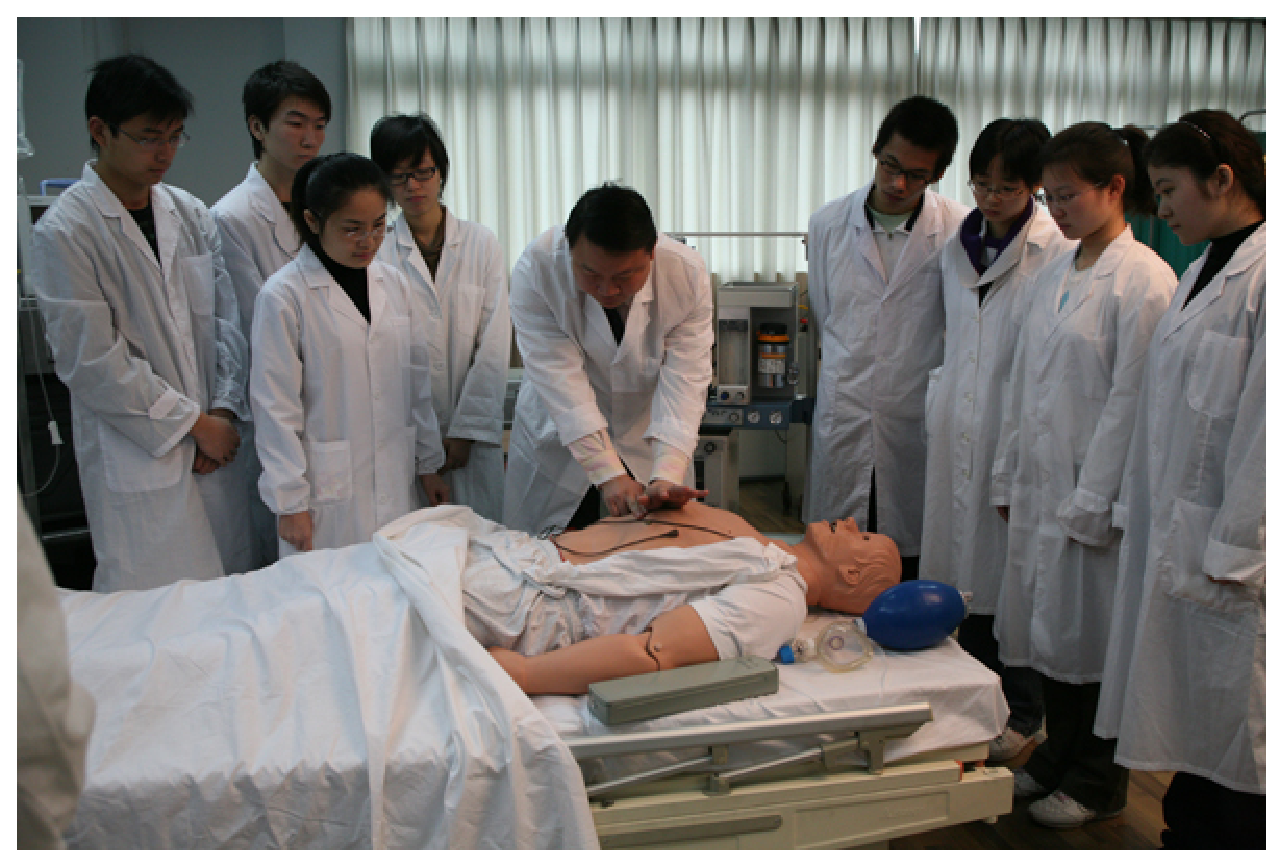
\includegraphics[height=70pt]{../../Figures/background/clinical_training_center.eps}
\quad
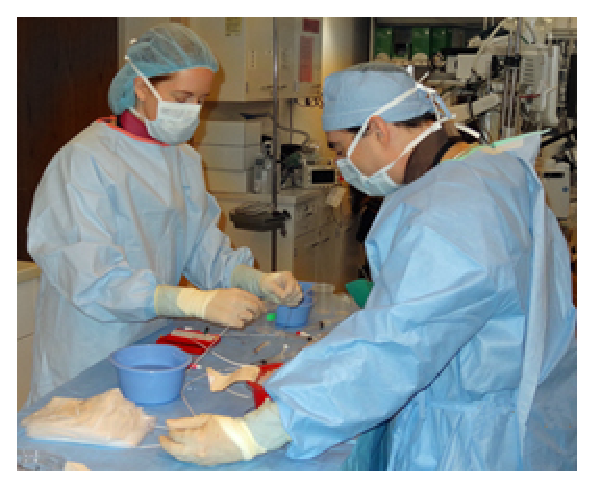
\includegraphics[height=70pt]{../../Figures/background/cath_lab.eps}
% }	
% \end{minipage}
\end{figure}
% \end{frame}

% \begin{frame}
\begin{itemize}
  \item \textbf{传统手术训练的缺点}:
  \begin{enumerate}
    \onslide<2-5> \item 不熟练的操作给病患带来的风险
    \onslide<3-5> \item 现场学习带来的不必要放射性危害
    \onslide<4-5> \item 机会宝贵,且无法复现
    \onslide<5> \item 严格受限于时间和地点
  \end{enumerate}
\end{itemize}
\end{frame}

% \begin{frame}
% \begin{itemize}
  % \item \textbf{微创血管介入手术机器人系统~[Ji(2011)]}: 
  % \begin{enumerate}
    % \onslide<1-2> \item 机器人系统外观
    % \onslide<2>\item 机器人控制系统
  % \end{enumerate}
% \end{itemize}
% \begin{columns}[b,onlytextwidth]
% \begin{column}{.5\textwidth}
% \onslide<1-2>\begin{figure}[t]
% \centering
% 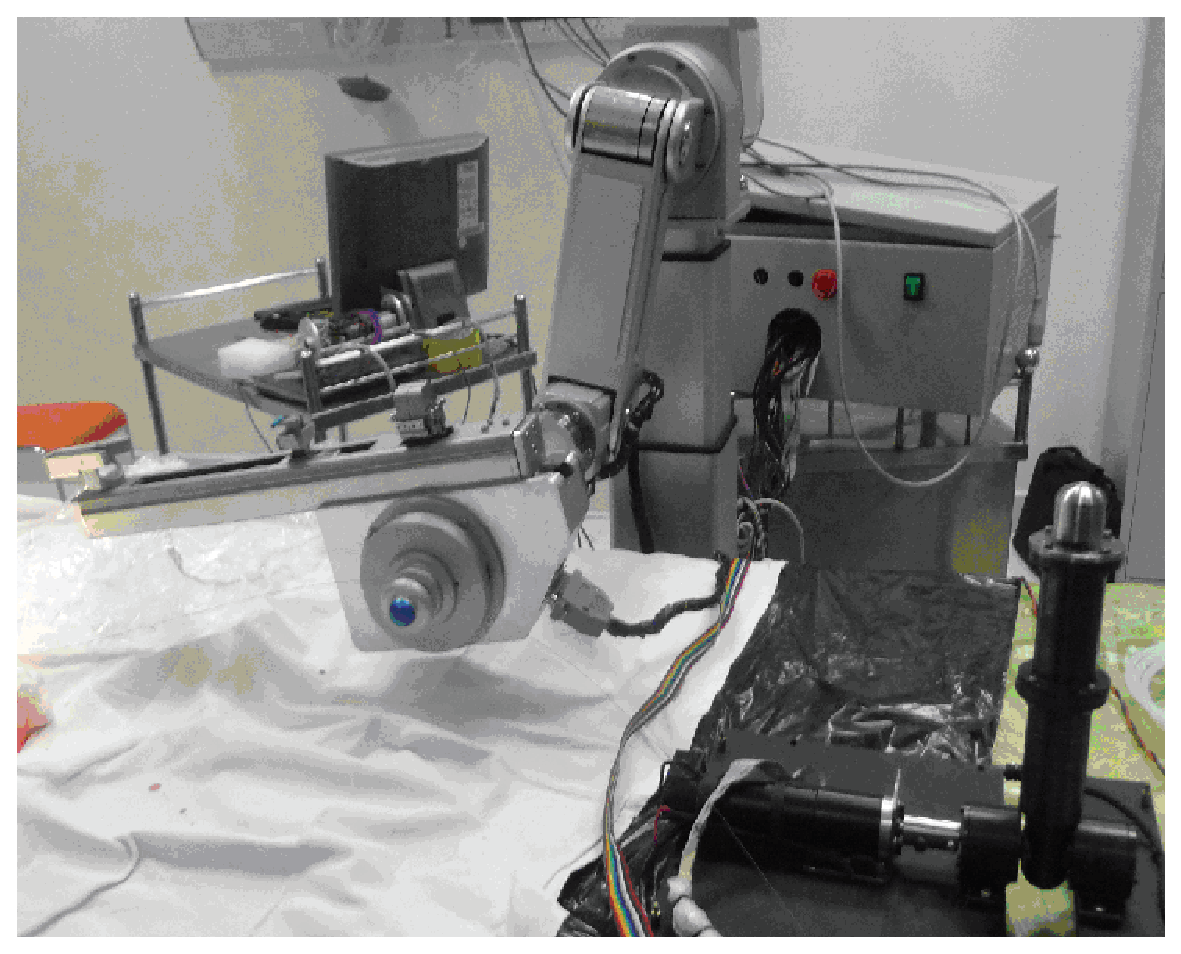
\includegraphics[height=100pt]{../../Figures/background/robot.eps}
% \end{figure}
% \end{column}
% \begin{column}{.5\textwidth}
% \onslide<2> \begin{figure}[t]
% \centering
% 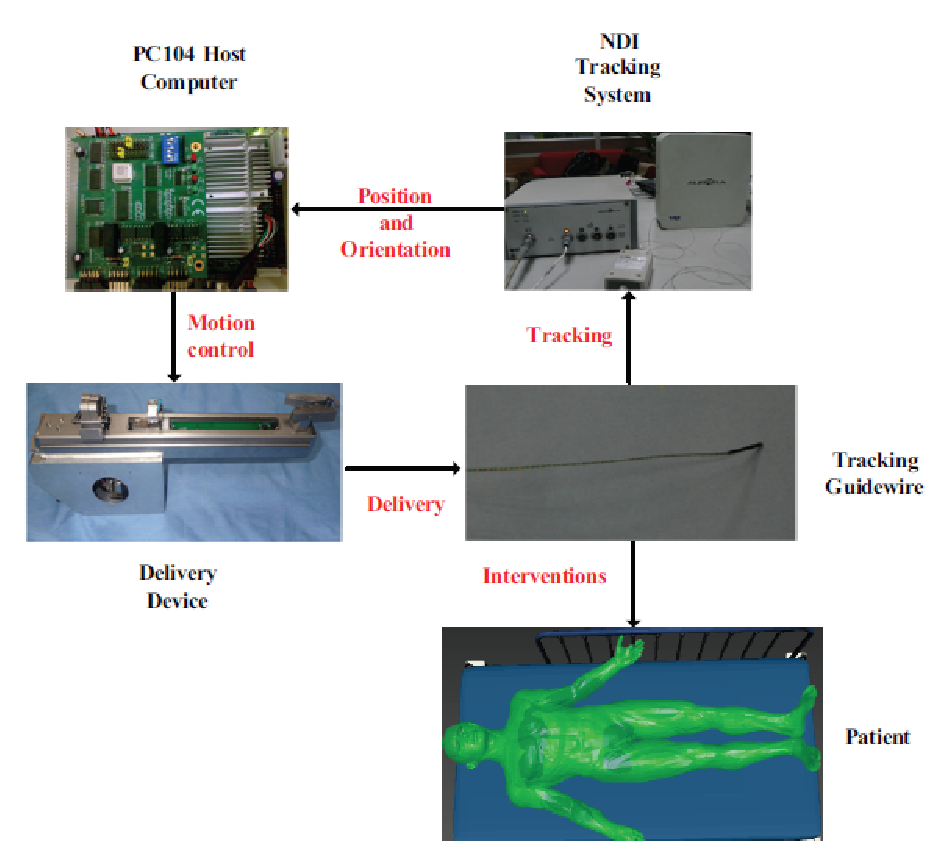
\includegraphics[height=100pt]{../../Figures/background/robot_arch.eps}
% \end{figure}
% \end{column}
% \end{columns}
% \end{frame}

\begin{frame}
\begin{itemize}
  \item \textbf{微创血管介入术仿真系统的基本配置}: 
  % \begin{enumerate}
    % \item 机器人外观
    % \item 机器人控制系统
  % \end{enumerate}
\end{itemize}
% \begin{columns}[b,onlytextwidth]
% \begin{column}{.5\textwidth}
\begin{figure}[t]
\centering
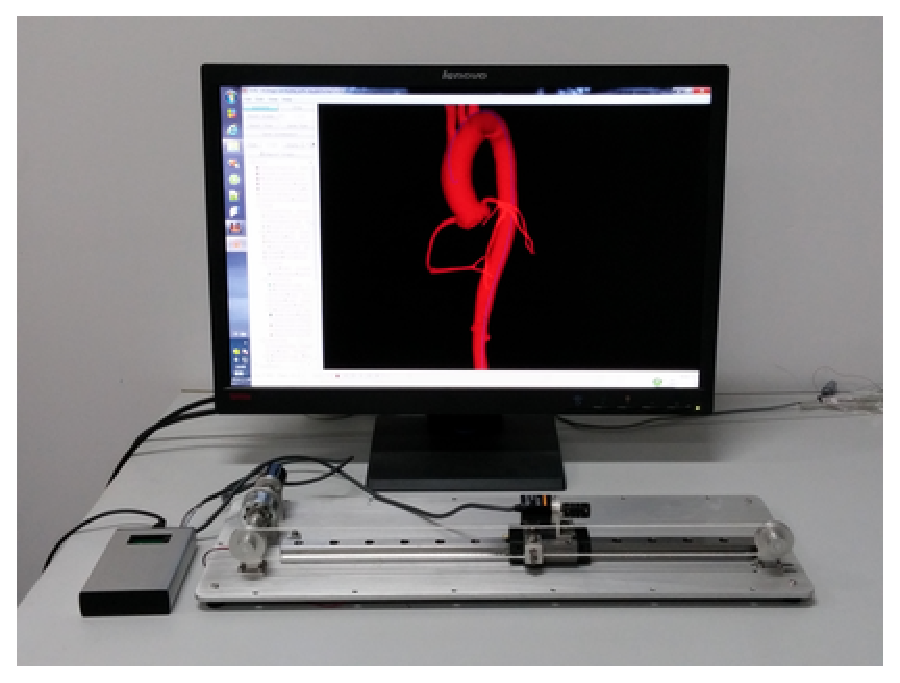
\includegraphics[height=130pt]{../../Figures/background/simulator.eps}
\end{figure}
% \end{column}
% \begin{column}{.5\textwidth}
% \begin{figure}[t]
% \centering
% \input{../../FigureSrc/background/architecture_utf8}
% \end{figure}
% \end{column}
% \end{columns}
\end{frame}

\begin{frame}
\begin{itemize}
  \item \textbf{微创血管介入术仿真系统的主要功能}: 
  \begin{enumerate}
    \onslide<1-5> \item 虚拟解剖环境
    \onslide<2-5> \item 虚拟手术工具
    \onslide<5> \item 触觉接口装置
  \end{enumerate}
\end{itemize}
\begin{columns}[b,onlytextwidth]
\begin{column}{.25\textwidth}
\onslide<3-5> \begin{figure}[t]
\centering
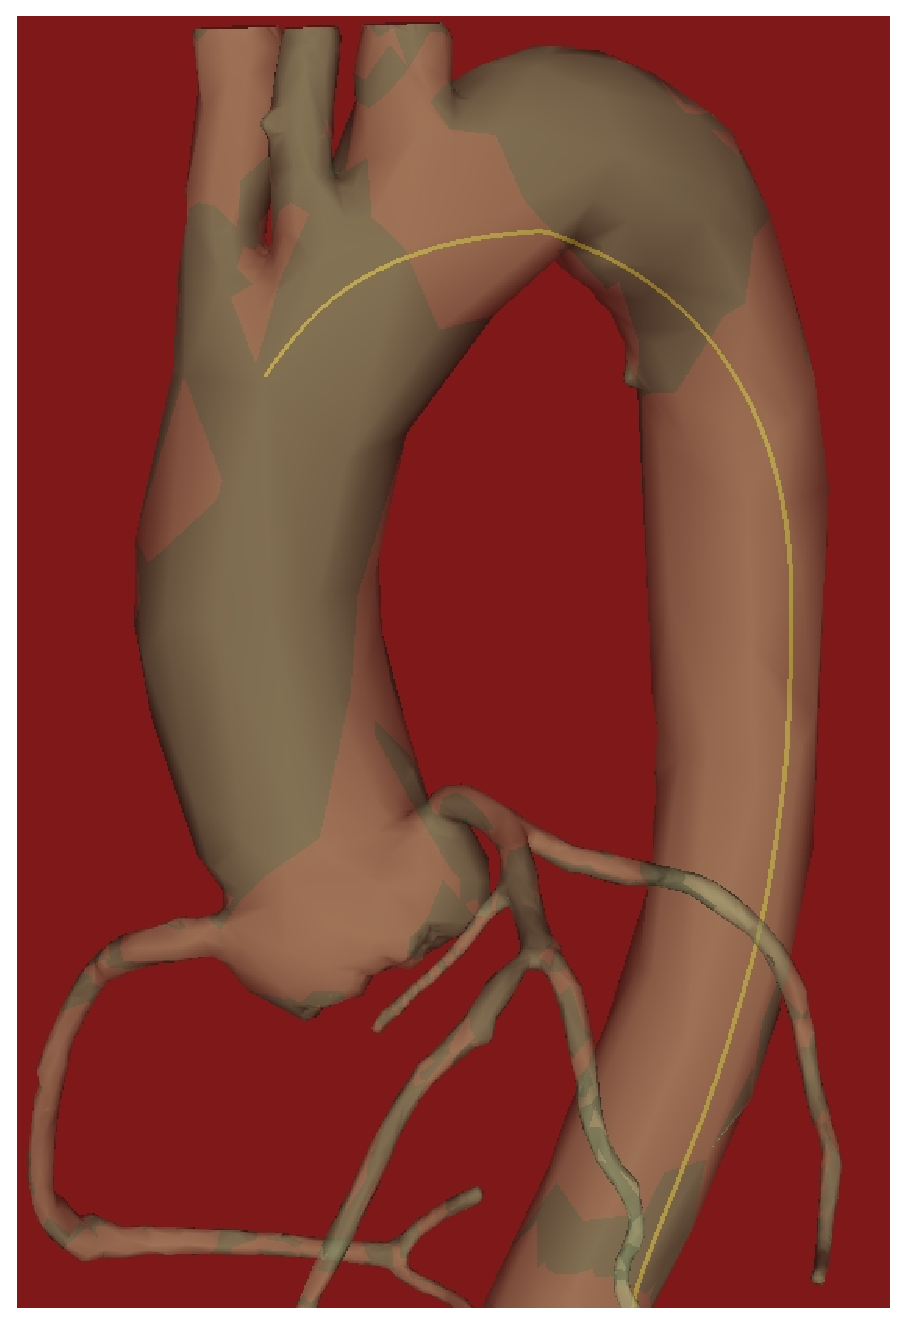
\includegraphics[height=1.0in]{../../Figures/background/simulation2.eps}
% 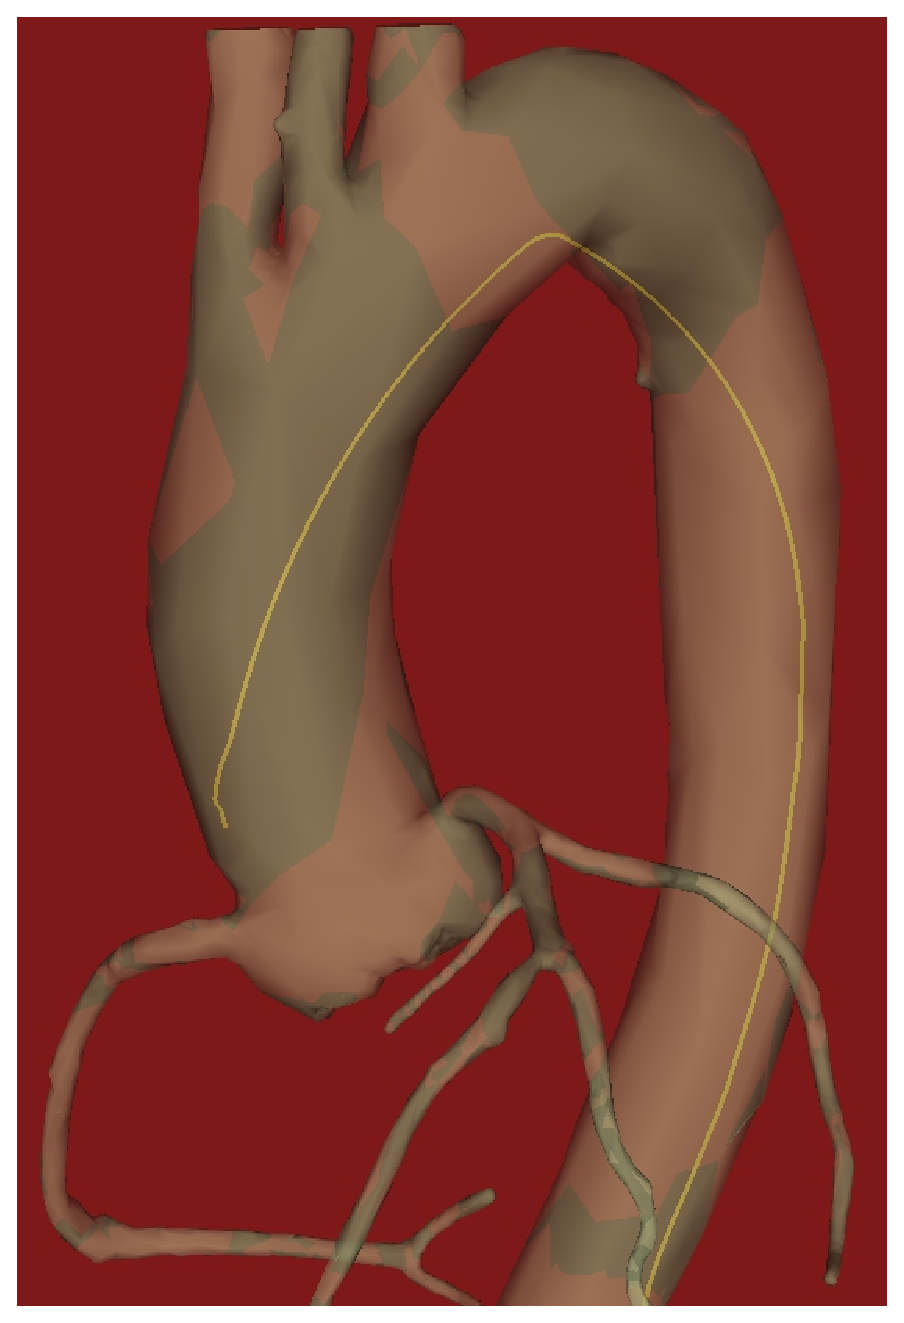
\includegraphics[height=1.0in]{../../Figures/background/simulation.eps}
% 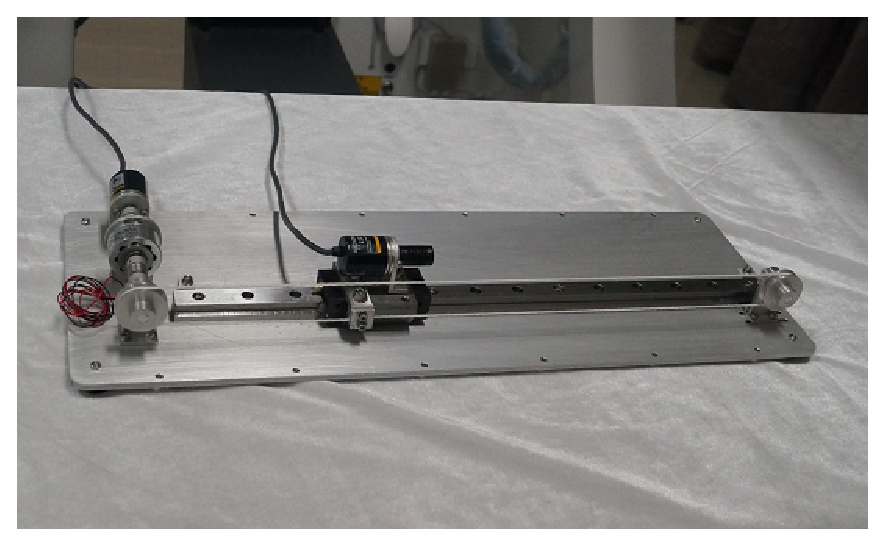
\includegraphics[height=1.0in]{../../Figures/background/interface.eps}
\end{figure}
\end{column}
\begin{column}{.25\textwidth}
\onslide<4-5> \begin{figure}[t]
\centering
% 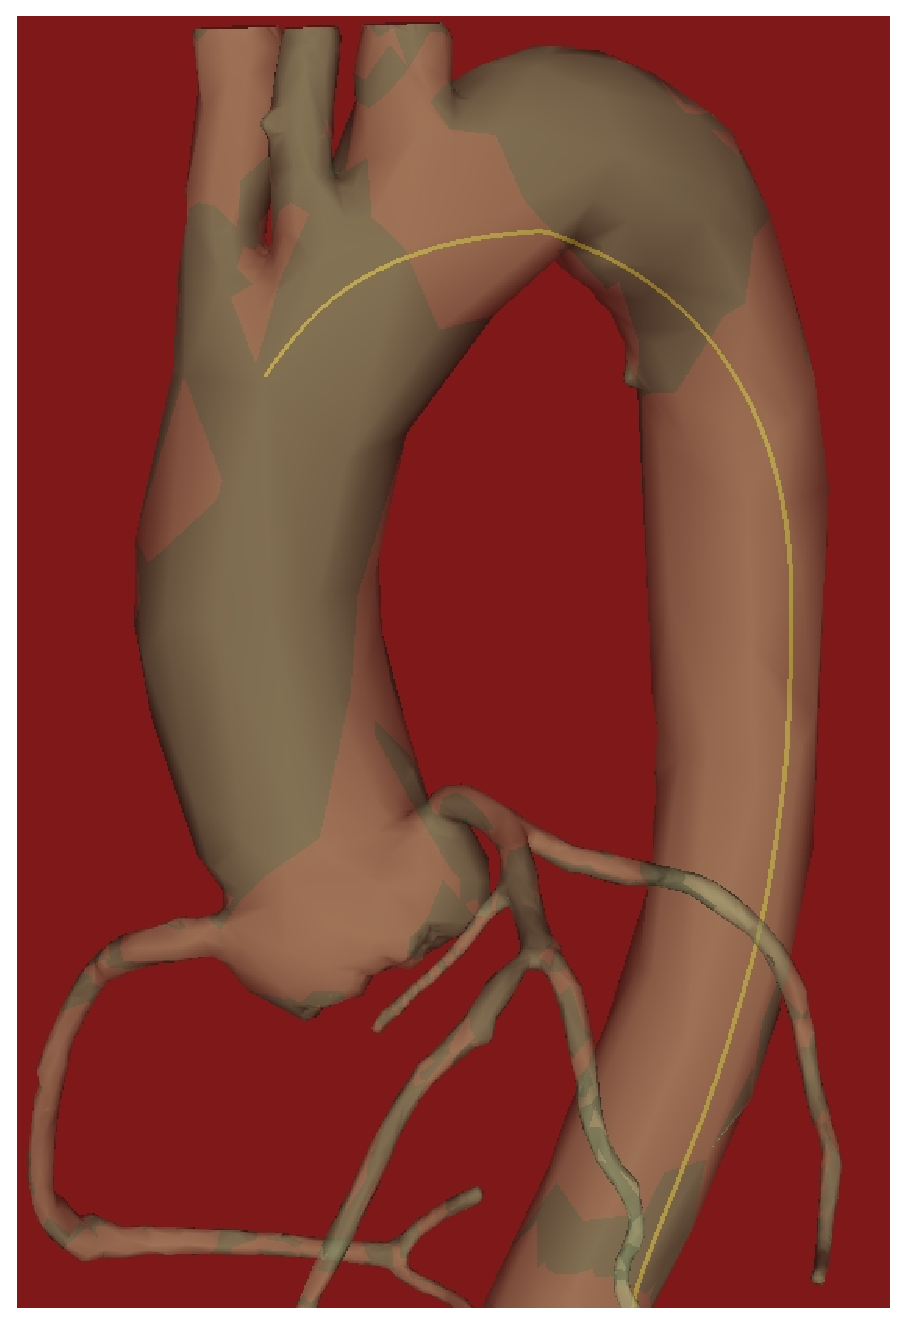
\includegraphics[height=1.0in]{../../Figures/background/simulation2.eps}
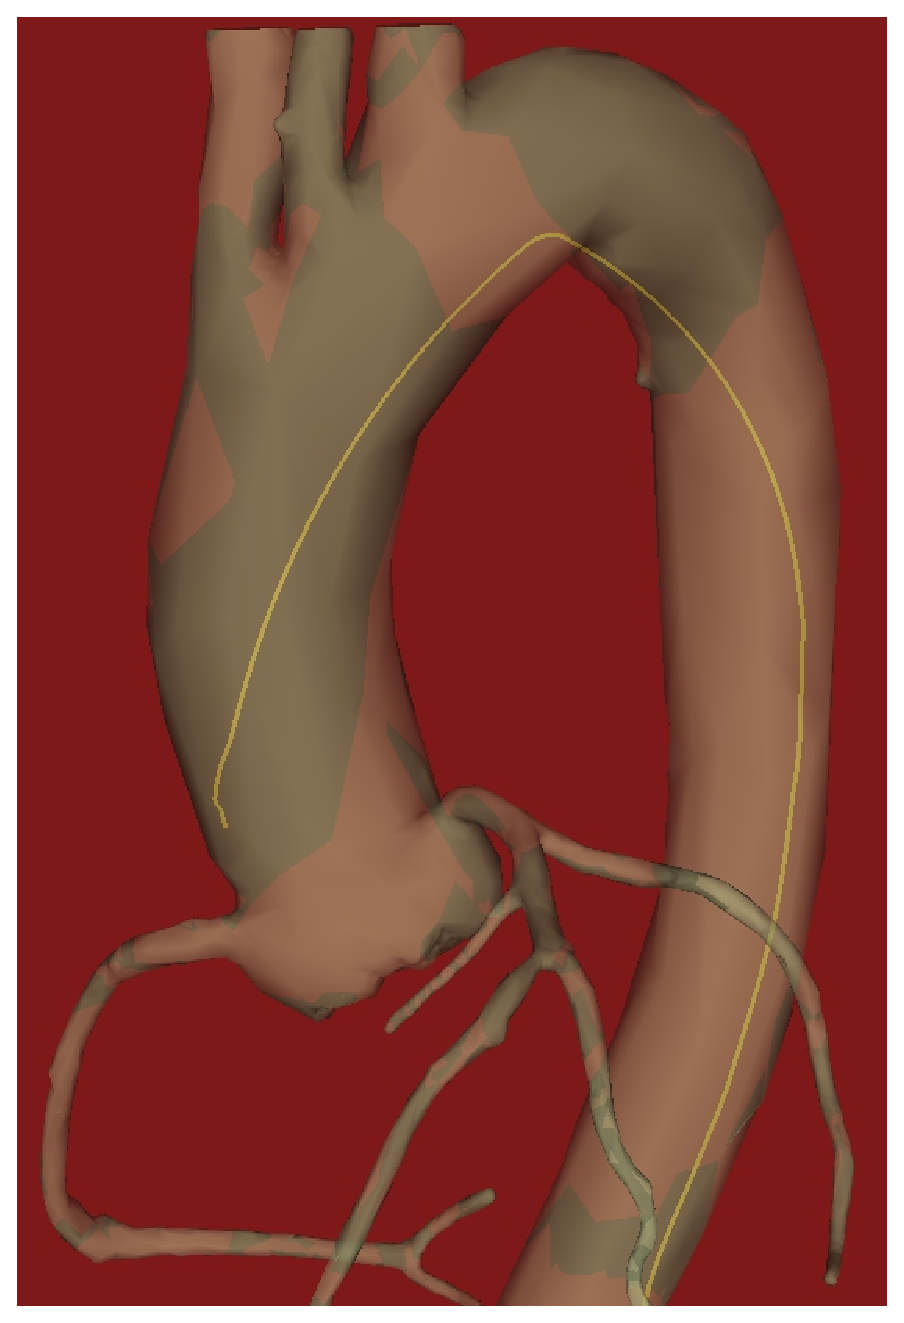
\includegraphics[height=1.0in]{../../Figures/background/simulation.eps}
% 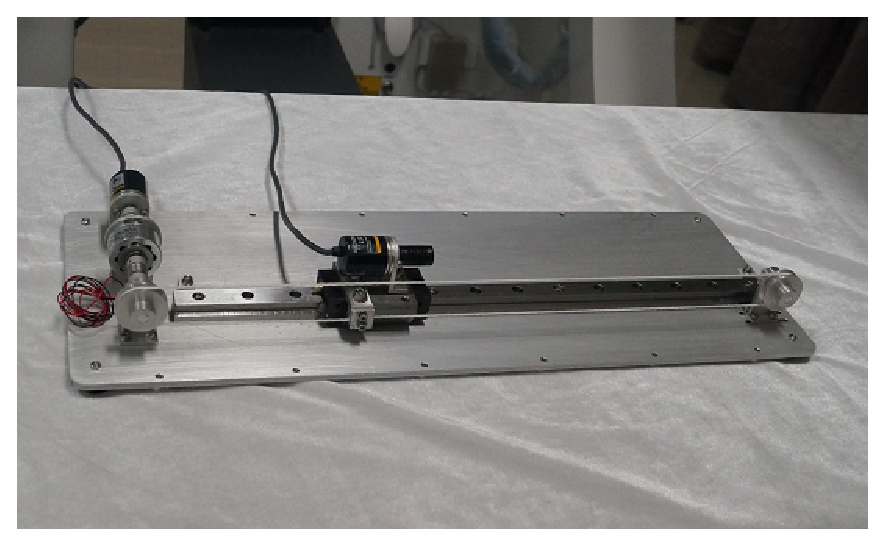
\includegraphics[height=1.0in]{../../Figures/background/interface.eps}
\end{figure}
\end{column}
\begin{column}{.5\textwidth}
\onslide<5> \begin{figure}[t]
\centering
% 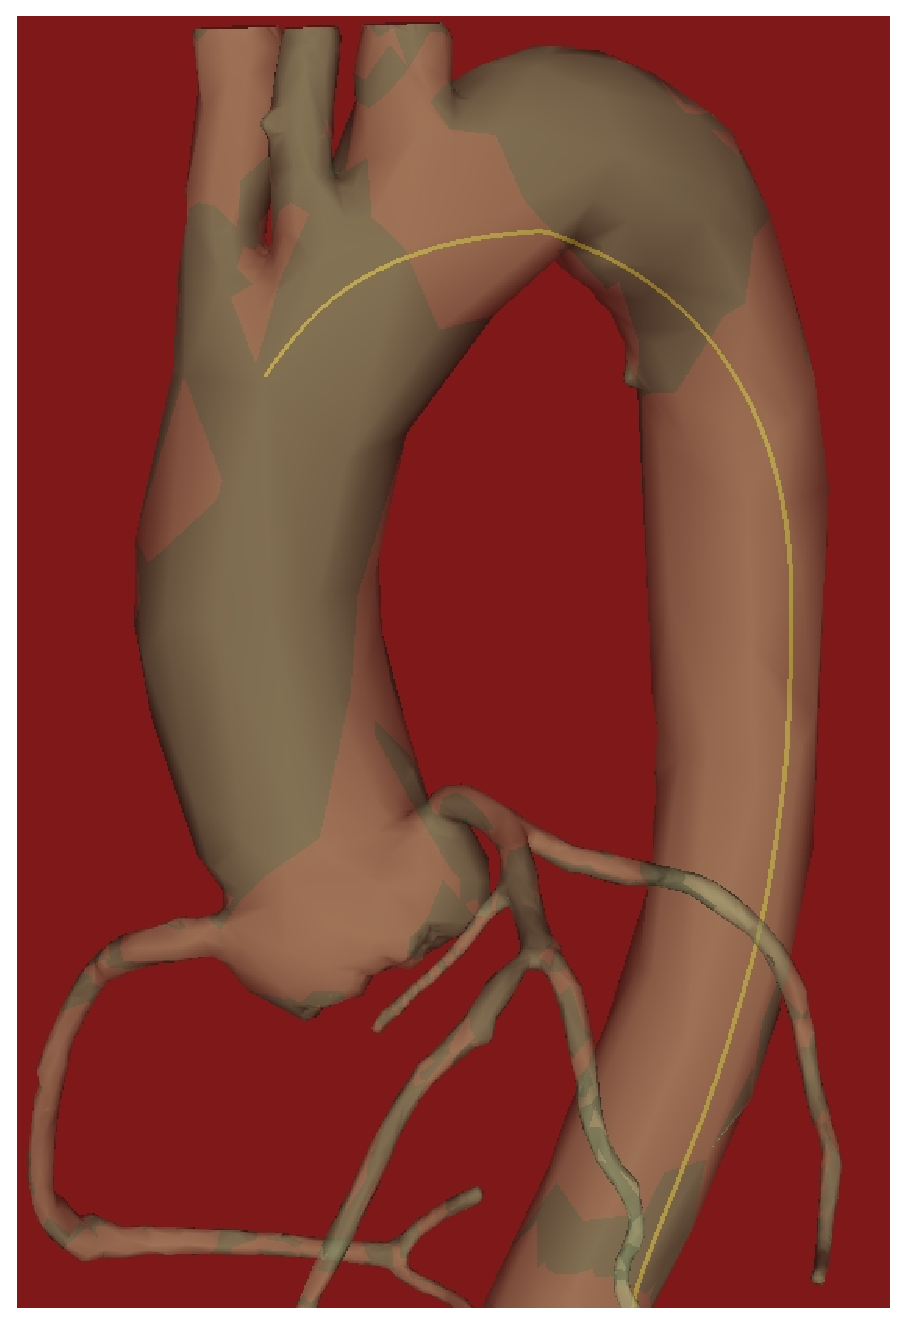
\includegraphics[height=1.0in]{../../Figures/background/simulation2.eps}
% 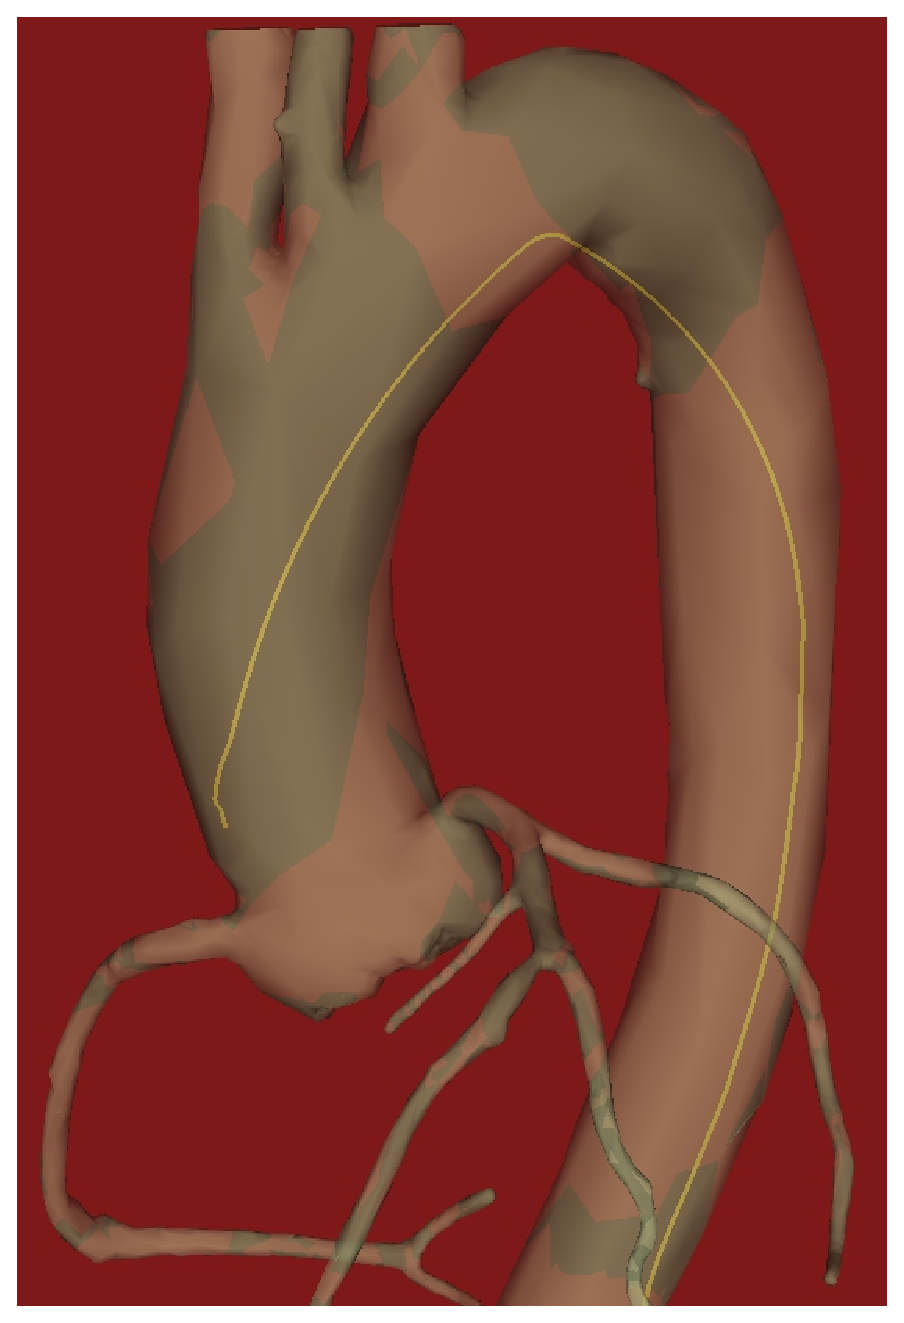
\includegraphics[height=1.0in]{../../Figures/background/simulation.eps}
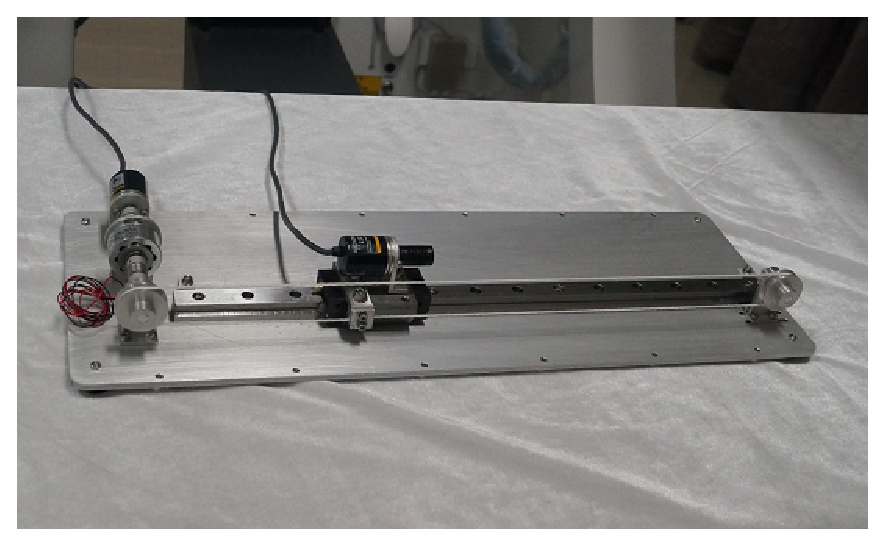
\includegraphics[height=1.0in]{../../Figures/background/interface.eps}
\end{figure}
\end{column}
\end{columns}
\end{frame}

\begin{frame}
\begin{itemize}
  \item \textbf{计算机仿真手术训练的优点}:
  \begin{enumerate}
    \onslide<1-5> \item 无不熟练操作风险
    \onslide<2-5> \item 无放射性危害
    \onslide<3-5> \item 可回放或重复操作过程
    \onslide<4-5> \item 无时间和地点的限制,可随时展开训练
    \onslide<5> \item 节省医疗资源
	\begin{itemize}
	\item 资深医生工时,手术器械,消毒间,等
	\end{itemize}
  \end{enumerate}
\end{itemize}
\end{frame}

\begin{frame}
\begin{itemize}
\item \textbf{技术难点}
\begin{itemize}
\pause \item 影像中主动脉与脊椎间隙过小甚至接触
\pause \item 影像中冠状动脉的亮度较暗,且走向多变,直径较小
\pause \item 心脏搏动导致心脏区域成像效果较差,无法准确提取完整模型
\pause \item 重建的表面模型数据量大,影响交互仿真的流畅度
\pause \item 重建的表面模型难以进行几何信息提取运算
\end{itemize}
\end{itemize}
\end{frame}

\begin{frame}
\begin{itemize}
  \item \textbf{本文贡献}
  \begin{itemize}
    \onslide<1-3> \item \textbf{基于真实病例数据的人心血管模型的创建}
    \begin{itemize}
      \onslide<2-3> \item 提出创建主动脉内腔模型的处理流程
      \onslide<2-3> \item 提出创建冠状动脉主要分支模型的处理流程
      \onslide<2-3> \item 提出创建冠状动脉次级分支模型的处理流程
      \onslide<2-3> \item 提出创建心脏近似模型的处理流程
    \end{itemize}
    \onslide<1-3> \item \textbf{面向交互仿真的人心血管模型的后处理}
    \begin{itemize}
      \onslide<3> \item 提出面向交互仿真的模型优化处理流程
      \onslide<3> \item 提出面向虚拟训练的模型几何信息提取处理流程
    \end{itemize}
  \end{itemize}
\end{itemize}
\end{frame} 